\documentclass[a4paper, 12pt]{report}
\usepackage[utf8]{inputenc}
\usepackage[IL2]{fontenc}
\usepackage[czech]{babel}
\usepackage{hyperref}
\usepackage{amsmath}
\usepackage{numprint}
\usepackage{graphicx}
\usepackage{listings}

\graphicspath{{img/}}

\lstset{language=C, columns=fullflexible, morekeywords={size_t, htab, nbc}}

\title{Identifikace spamu naivním bayesovským klasifikátorem}
\author{Stanislav Kafara}
\date{\today}

\begin{document}

\begin{titlepage}

\begin{center}

\begin{figure}
\centering

\includegraphics[width=.75\textwidth]{FAV_logo}
%\caption{Logo Fakulty aplikovaných věd ZČU}
%\label{fig:fav_logo}
\end{figure}

\vspace{4\baselineskip}

Semestrální práce z~předmětu\\
Programování v~jazyce C

\vspace{2\baselineskip}

{\makeatletter
\LARGE \bfseries \@title
\makeatother}

\end{center}

\vfill

\begin{flushleft}

\textbf{Autor:}\\
{\makeatletter
\@author
\makeatother}\\
A21B0160P\\
\texttt{skafara@students.zcu.cz}

\vspace{\baselineskip}

\textbf{Vyučující:}\\
Kamil Ekštein\\
\texttt{kekstein@kiv.zcu.cz}

\end{flushleft}

\end{titlepage}

\begin{tableofcontents}

\end{tableofcontents}

\chapter{Zadání}

Naprogramujte v~ANSI C přenositelnou\footnote{Je třeba, aby bylo možné Váš 
program přeložit a spustit na PC s~operačním prostředím Win32/64 (tj. 
operační systémy Microsoft Windows NT/2000/XP/Vista/7/8/10/11) a s~běžnými 
distribucemi Linuxu (např. Ubuntu, Debian, Red Hat, atp.). Server, na 
který budete Vaši práci odevzdávat a který ji otestuje, má nainstalovaný 
operační systém Debian GNU/Linux 10 (buster) s~jádrem verze 
4.19.0-11-amd64 a s~překladačem gcc 8.3.0.} \textbf{konzolovou aplikaci}, 
která bude \textbf{rozhodovat, zda úsek textu} (textový soubor předaný 
jako parametr na příkazové řádce) \textbf{je nebo není spam}.

Program bude přijímat z~příkazové řádky celkem \textbf{sedm} parametrů: 
První dva parametry budou vzor jména a počet trénovacích souborů 
obsahujících nevyžádané zprávy (tzv. \textbf{spam}). Třetí a čtvrtý 
parametr budou vzor jména a počet trénovacích souborů obsahujících 
vyžádané zprávy (tzv. \textbf{ham}). Pátý a šestý parametr budou vzor 
jména a počet testovacích souborů. Sedmý parametr představuje jméno 
výstupního textového souboru, který bude po dokončení činnosti Vašeho 
programu obsahovat výsledky klasifikace testovacích souborů.

Program se tedy bude spouštět příkazem

\texttt{spamid.exe\footnote{Přípona \texttt{.exe} je povinná i při 
sestavení v~Linuxu, zejm. při automatické kontrole validačním systémem.} 
⟨spam⟩ ⟨spam-cnt⟩ ⟨ham⟩ ⟨ham-cnt⟩ ⟨test⟩ ⟨test-\linebreak cnt⟩ ⟨out-file⟩}

Symboly ⟨\texttt{spam}⟩, ⟨\texttt{ham}⟩ a ⟨\texttt{test}⟩ představují 
vzory jména vstupních souborů. Symboly ⟨\texttt{spam-cnt}⟩, 
⟨\texttt{ham-cnt}⟩ a ⟨\texttt{test-cnt}⟩ představují počty vstupních 
souborů. Vstupní soubory mají následující pojmenování: \texttt{vzorN}, kde 
\texttt{N} je celé číslo z~intervalu ⟨$1;N$⟩. Přípona všech vstupních 
souborů je \texttt{.txt}, přípona není součástí vzoru. Váš program tedy 
může být během testování spuštěn například takto:

\texttt{spamid.exe spam 10 ham 20 test 50 result.txt}

Výsledkem činnosti programu bude textový soubor, který bude obsahovat 
seznam testovaných souborů a jejich klasifikaci (tedy rozhodnutí, zda je
o~spam či neškodný obsah – ham).

Pokud nebude na příkazové řádce uvedeno právě sedm argumentů, vypište 
chybové hlášení a stručný návod k~použití programu v~angličtině podle 
běžných zvyklostí (viz např. ukázková semestrální práce na webu předmětu 
Programování v~jazyce C). \textbf{Vstupem programu jsou pouze argumenty na 
příkazové řádce – interakce s~uživatelem pomocí klávesnice či myši
v~průběhu práce programu se neočekává.}

Hotovou práci odevzdejte v~jediném archivu typu ZIP prostřednictvím 
automatického odevzdávacího a validačního systému. Postupujte podle 
instrukcí uvedených na webu předmětu. Archiv nechť obsahuje všechny 
zdrojové soubory potřebné k~přeložení programu, \textbf{makefile} pro 
Windows i Linux (pro překlad v~Linuxu připravte soubor pojmenovaný 
\texttt{makefile} a pro Windows \texttt{makefile.win}) a dokumentaci ve 
formátu PDF vytvořenou v~typografickém systému \TeX, resp. \LaTeX. Bude-li 
některá z~částí chybět, kontrolní skript Vaši práci odmítne.

\chapter{Analýza úlohy}

Program má postupovat ve dvou fázích. Nejdříve nechá trénovacími soubory 
natrénovat klasifikátor, kterým následně klasifikuje testované soubory. 
Úloha se skládá z~několika problémů, které je nutné analyzovat a jimiž 
jsou:

\begin{itemize}
    \item čtení slov ze souborů,
    \item trénování,
    \item klasifikace a
    \item reprezentace dat.
\end{itemize}

V~této kapitole je odkazováno na zadání 
práce\footnote{\texttt{https://www.kiv.zcu.cz/studies/predmety/pc/data/works/sw2022-02.pdf}}.

\section{Datové soubory}

Datové soubory obsahují právě jednu řádku mezerou oddělených slov, a tak 
není potřeba je nijak předzpracovávat. Je ale potřeba zamyslet se nad tím, 
kdy a jak budou slova ze souborů načítána.

Je možné zvolit mezi přístupy načtení slov ze souborů dopředu, a nebo 
načítání slov ze souborů během trénování. Pokud by byly datové soubory 
příliš velké, načtená slova by se nemusela vejít do operační paměti, čemuž 
se dá částečně zabránit druhým přístupem, který bude využíván.

Další věc, nad kterou je potřeba se zamyslet, je maximální délka slova. 
Pokud by datové soubory obsahovaly slova přirozených jazyků, pro načtení 
slova by postačovala statická vyrovnávací paměť o~určité velikosti. Jinou 
možností může být např. nejprve analyzovat datový soubor a následně
s~pomocí dynamické alokace vytvořit dostatečně velkou vyrovnávací paměť. Pro 
jednoduchost bude zvolen přístup načítání slova do dynamického pole, který 
může být využit i v~případě, že datové soubory obsahují řetězce jiného 
významu, než slova přirozeného jazyka a ze souboru je tak čteno pouze 
jednou.

\section{Trénování}
\label{text:analysis-nbc-learn}

Natrénováním naivního Bayesovského klasifikátoru se rozumí vypočtení 
hodnot pro každou klasifikační třídu tohoto modelu, na základě nichž model 
následně klasifikuje testované datové soubory. Těmito hodnotami jsou 
$P(c)$ a $P(\langle \text{word} \rangle|c)$ a jsou vypočteny podle vzorce 
\ref{equ:nbc-class-probability} a \ref{equ:nbc-word-class-probability}.

$P(c)$ je apriorní pravděpodobnost výskytu klasifikační třídy $c$
v~datových souborech. $P(\langle \text{word} \rangle|c)$ je pravděpodobnost 
výskytu slova ⟨word⟩ v~datovém souboru za podmínky klasifikace datového 
souboru do klasifikační třídy $c$. Klasifikátor využívá tzv. 
\textit{bag-of-words model}\footnote{Nepracuje se s~pozicí výskytu slova
v~datovém souboru, nýbrž jen se skutečností jeho výskytu v~něm.}.

\begin{equation}
    P(c_i) = \frac{|\text{\textbf{doc}}_i|}{|\text{\textbf{trénovací 
množina}}|}
    \label{equ:nbc-class-probability}
\end{equation}

\begin{equation}
    P(\langle \text{word} \rangle|c_i) = \frac{n_k + 1}{n + 
|\text{\textbf{slovník}}|}
    \label{equ:nbc-word-class-probability}
\end{equation}

Symbol $c_i$ představuje $i$-tou klasifikační třídu, 
$|\text{\textbf{doc}}_i|$ počet datových souborů patřící do $i$-té 
klasifikační třídy, $|\text{\textbf{trénovací množina}}|$ celkový počet 
trénovacích datových souborů, ⟨word⟩ slovo, $n$ počet slov (včetně 
duplicitních) v~datových souborech patřících do $i$-té klasifikační třídy, 
$n_k$ počet slov ⟨word⟩ v~datových souborech patřících do $i$-té 
klasifikační třídy a $|\text{\textbf{slovník}}|$ počet různých slov ve 
všech trénovacích datových souborech.

Lze vybírat mezi přístupy postupného trénování a přepočítávání 
pravděpodobností a nebo jednorázového natrénování několika datových 
souborů a jednorázového vypočtení pravděpodobností. Přístupy lze také 
kombinovat. První přístup v~této úloze nenajde uplatnění, a samotný navíc 
zvyšuje časovou složitost trénování, proto bude využíván přístup druhý.

\section{Klasifikace}
\label{text:analysis-nbc-classify}

Klasifikací datového souboru se rozumí přiřazení klasifikační třídy 
datovému souboru. Naivní Bayesův klasifikátor přiřazuje datovému souboru 
klasifikační třídu $c$ na základě pravděpodobností vypočtených během 
trénování podle vzorce \ref{equ:nbc-classification-mathematical}.

\begin{equation}
    c = \arg\max_{c_i \in C} \left( P(c_i) \cdot \prod_{k \in 
\text{\textbf{pozice}}} P(\langle \text{word}_k \rangle|c_i) \right),
    \label{equ:nbc-classification-mathematical}
\end{equation}

kde $C$ je množina klasifikačních tříd (v~této úloze pouze spam a ham), 
\textbf{pozice} je množina pozic slov v~testovaném datovém souboru 
takových, že slovo na této pozici je ve slovníku klasifikátoru (nacházelo 
se v~nějakém z~trénovacích datových souborů) a $\langle \text{word}_k 
\rangle$ je $k$-té slovo testovaného datového souboru. Avšak z~důvodu 
možnosti podtečení rozsahu čísel s~pohyblivou desetinnou čárkou je 
využívána zlogaritmovaná verze vzorce \ref{equ:nbc-classification-real}.

\begin{equation}
    c = \arg\max_{c_i \in C} \left( \log P(c_i) + \sum_{k \in 
\text{\textbf{pozice}}} \log P(\langle \text{word}_k \rangle|c_i) \right).
    \label{equ:nbc-classification-real}
\end{equation}

\section{Reprezentace dat klasifikátoru}

Pro efektivní natrénování klasifikátoru a klasifikaci datových souborů je 
potřeba využít datovou strukturu poskytující přidání prvku a získání prvku 
se vhodnou časovou a paměťovou složitostí.

\subsection{Využití datové struktury}

K~natrénování klasifikátoru je nutné provést $2 \cdot 
|\text{\textbf{slovník}}|$ výpočtů pravděpodobnosti $P(\langle \text{word} 
\rangle|c)$ podle vzorce \ref{equ:nbc-word-class-probability}, proto je 
potřeba mít hodnoty efektivně dostupné pro dosazení do vzorce.

Ke klasifikaci datového souboru podle vzorce 
\ref{equ:nbc-classification-real} je nutné provést 2 komplexní výpočty 
vyžadující $|\text{\textbf{slovník}}|$krát získání a dosazení hodnoty 
pravděpodobnosti $P(\langle \text{word} \rangle|c)$ do vzorce.

\subsection{Vhodná datová struktura}

Nabízí se řešit problém pomocí hash tabulky, prefixové trie nebo binárního 
(případně i vyvažovaného) vyhledávacího stromu.

Paměťová složitost vybraných datových struktur je shodná v~nejhorším 
případě. V~průměrném případě by nejvhodnější volbou byla prefixová trie, 
potom hash tabulka a binárná vyhledávací strom.

Časová složitost vkládání prvku a získání prvku závisí u~hash tabulky jen 
na délce řetězce, u~trie navíc na počtu písmen abecedy jazyka a
u~binárního vyhledávacího stromu navíc ještě na počtu již vložených prvků
v~datové struktuře.

Pro očekávané vlastnosti hash tabulky je potřeba zajistit nejlépe 
rovnoměrné rozptýlení vkládaných prvků, řešení případných kolizí a 
přiměřenou velikost tabulky, nejlépe rovnu prvočíslu.

Z~důvodu předpokladu zvýhodnění časové složitosti nad paměťovou složitostí 
a jednoduchosti implementace je zvolena datová struktura hash tabulka
s~dynamickou velikostí a s~využitím rychlého testu prvočíselnosti.

\chapter{Popis implementace}

Zjednodušená adresářová struktura projektu s~ukázkovými daty je vidět na 
obr. \ref{fig:project-tree-simplified}. Zdrojové kódy programu se nachází 
v~adresáři \texttt{src} a datové soubory v~adresáři \texttt{data}.
V~adresáři \texttt{doc/html} je dostupná vygenerovaná programová dokumentace 
programem \texttt{doxygen} ve formátu HTML.

\begin{figure}
    \centering
    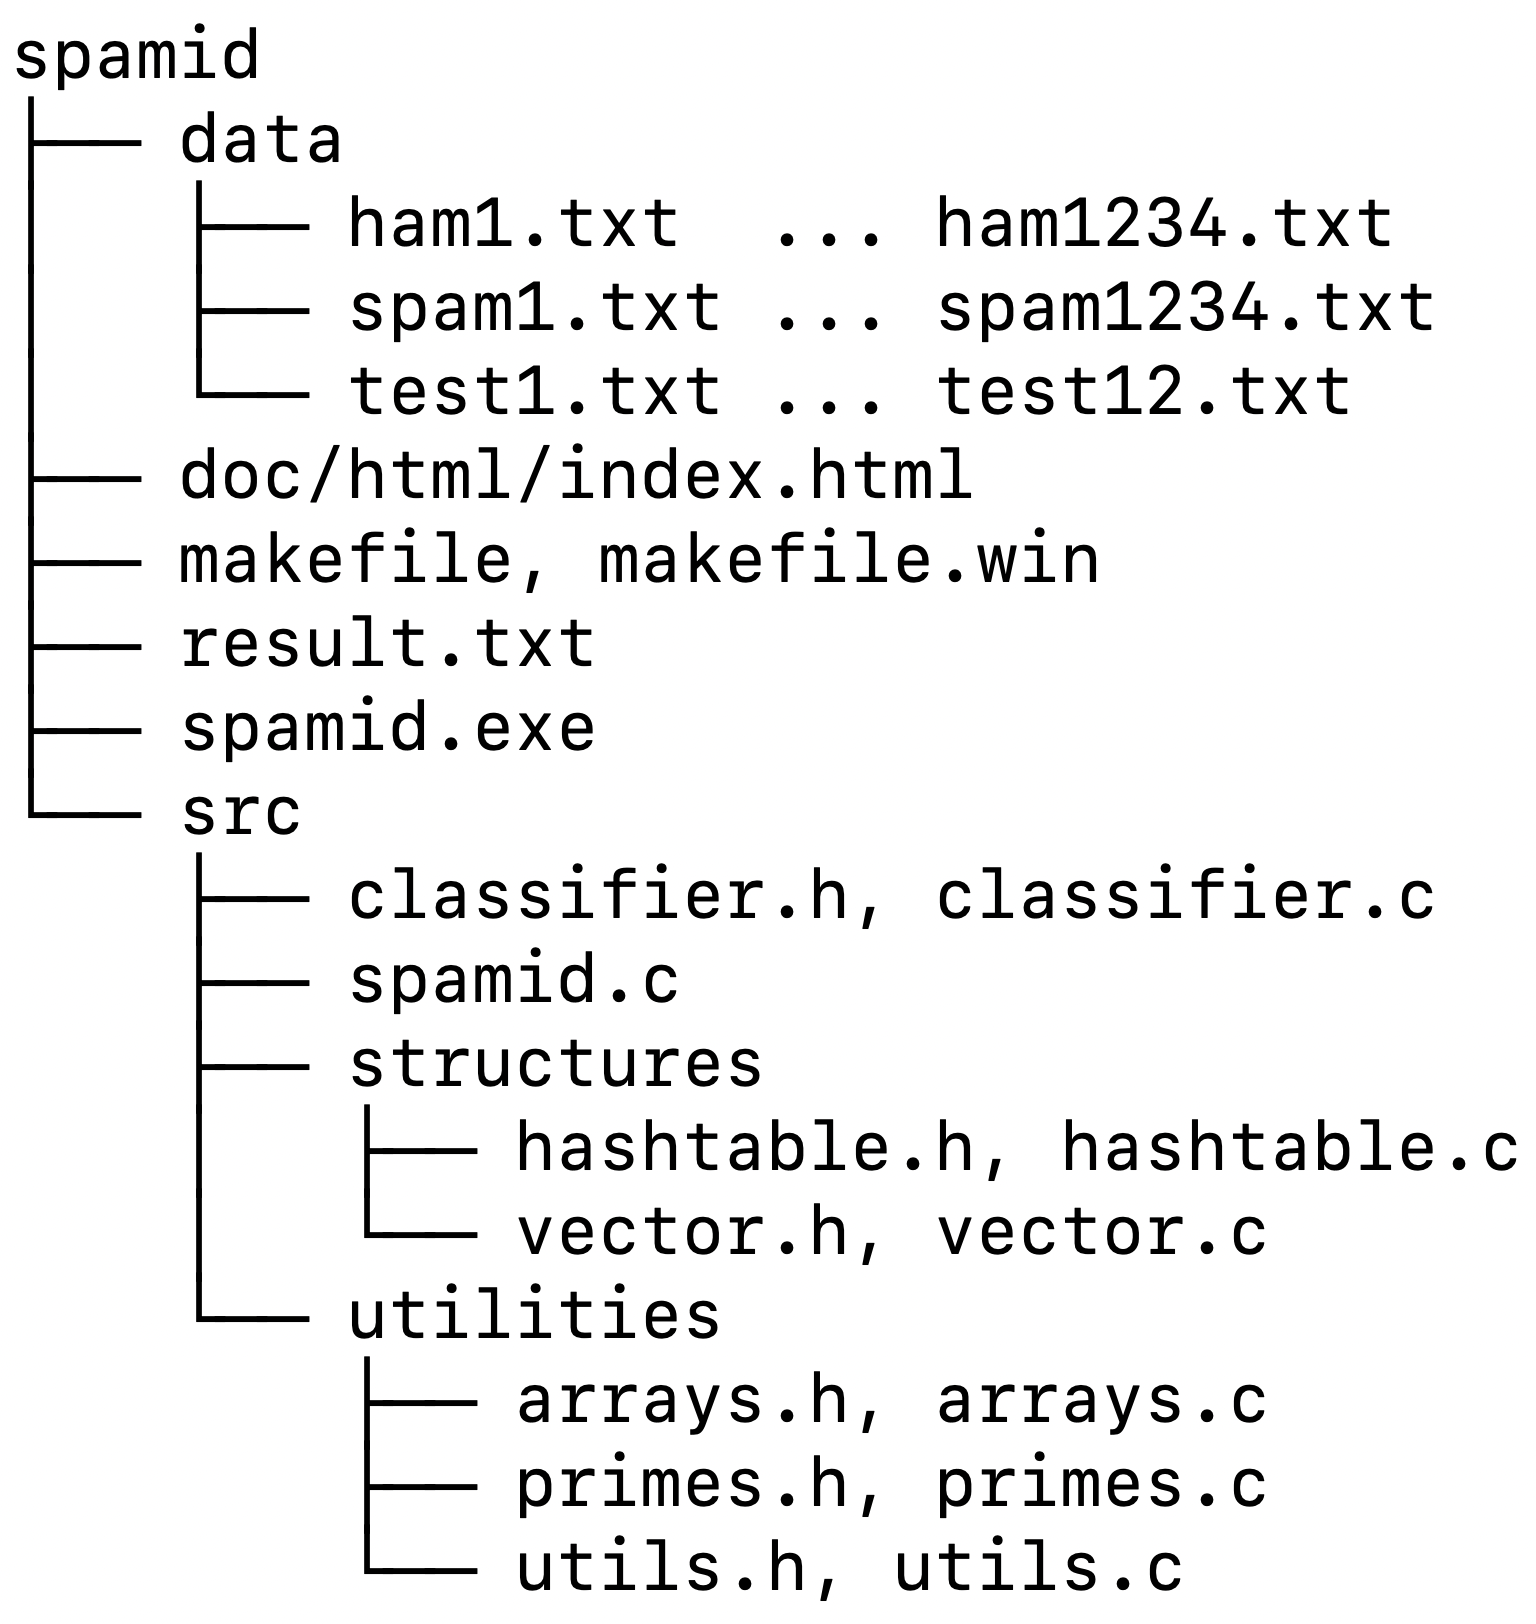
\includegraphics[width=.75\textwidth]{project-tree-simplified}
    \caption{Zjednodušená adresářová struktura projektu s~ukázkovými daty}
    \label{fig:project-tree-simplified}
\end{figure}

Zdrojový kód programu je dělen podle významových bloků do balíků a modulů. 
Deklarace funkcí implementovaných moduly se nachází ve stejnojmenných 
hlavičkových souborech.

\section{Balík \texttt{utilities}}

V~balíku se nachází moduly obsahující především pomocné funkce pro vyšší 
vrstvy programu.

\subsection{Modul \texttt{utils}}

Obsahem modulu je jediná funkce \texttt{strdup}, která není standardem 
ANSI~C podporována. Funkce duplikuje řetězec tak, že dynamicky alokuje 
nový paměťový prostor a do něj řetězec překopíruje.

\subsection{Modul \texttt{primes}}

Modul poskytuje funkce pro test prvočíselnosti a získání dalšího 
prvočísla.

Pro test prvočíselnosti je využíván Millerův-Rabinův test prvočíselnosti. 
Pro čísla menší než \numprint{1373653} je zvolena efektivní 
deterministická varianta testu, pro jiná čísla se jedná o~standardní test 
s~$\approx~\numprint{99.998}\%$ úspěšností.

Získání dalšího prvočísla probíhá postupným testováním čísel zmíněným 
testem prvočíselnosti.

\subsection{Modul \texttt{arrays}}

V~modulu se nachází funkce pro jednoduchou práci se staticky i dynamicky 
alokovanými poli.

K~dispozici jsou funkce pro dynamické vytvoření pole, vymazání prvků pole, 
uvolnění paměti pole a získání extremálního prvku pole s~využitím 
deklarovaného komparátoru prvků pole.

\section{Balík \texttt{structures}}

Balík obsahuje moduly poskytující funkce pro práci s~využívanými datovými 
strukturami.

\subsection{Modul \texttt{vector}}

Obsahem modulu jsou funkce pro práci se staticky či dynamicky založeným 
dynamickým polem.

K~dispozici jsou funkce pro statické či dynamické vytvoření dynamického 
pole a uvolnění paměti dynamického pole s~možností uvolnění i jeho prvků
s~využitím deklarované funkce pro uvolňení paměti patřící prvku dynamického 
pole.

Dále obsahuje funkce pro přidání prvku nebo několika prvků, získání 
ukazatele na prvek na $i$-té pozici a přenechání dat.

Dalšími funkcemi v~modulu jsou funkce pro získání počtu prvků dynamického 
pole a navýšení nebo ponížení kapacity dynamického pole.

\subsection{Modul \texttt{hashtable}}

Modul obsahuje funkce pro práci s~dynamicky vytvořenou hash tabulkou a 
dynamicky vytvořeným iterátorem nad prvky hash tabulky.

Poskytnuty jsou funkce pro dynamické založení hash tabulky a uvolnění 
paměti hash tabulky s~možností uvolnění i jejich prvků (hodnot) s~využitím 
deklarované funkce pro uvolnění paměti patřící prvku hash tabulky.

Dále jsou dostupné funkce pro přidání prvku do hash tabulky, zjištění 
existence klíče v~hash tabulce, získání hodnoty nebo ukazatele na hodnotu 
přiřazené klíči v~hash tabulce a získání počtu prvků v~hash tabulce.

Další možnost práce s~prvky hash tabulky je pomocí iterátoru. K~dispozici 
jsou funkce pro jeho dynamické vytvoření, uvolnění paměti, návrat na 
začátek a funkce pro zjištění existence dalšího prvku a získání dalšího 
prvku.

\subsubsection{Implementace hash tabulky}

Hash tabulka rozptyluje prvky do pole o~velikosti rovné prvočíslu 
spojových seznamů párů klíče a hodnoty na základě vypočteného hash kódu 
klíče.

Do hash tabulky se ukládá kopie klíče (řetězce) a kopie hodnoty (ukazatel na libovolný typ nebo přímo libovolná hodnota).

Velikost pole hash tabulky je prvočíselná a dynamická. Pokud nastane 
situace, že je vkládán nový prvek a počet prvků hash tabulky je roven 
pětinásobku velikosti pole, velikost pole se zvětší na prvočíslo nejbližší 
větší nebo rovno dvojnásobku aktuální velikosti pole, dosud vložené prvky 
jsou v~poli přeskládány podle aktuálních hash kódů jejich klíčů a do hash 
tabulky se vloží nový prvek. Tím je zachována časová složitost vložení 
prvku v~konstantním čase v~závislosti na počtu vkládaných prvků.

Prvkem pole hash tabulky je spojový seznam obsahující pár klíč a hodnota 
vkládaného prvku a ukazatel na další prvek spojového seznamu. V~průměrném 
případě je délka tohoto spojového seznamu nejvýše 5, tedy konstantní. Tím 
je zachována časová složitost získání prvku v~konstantním čase
v~závislosti na počtu vložených prvků.

Hash kód $h$ klíče $s$ (řetězce délky $n$ složeného z~písmen $s_0$ až 
$s_{n-1}$) je vypočten podle vzorce \ref{equ:htab-hcode} efektivně pomocí 
algoritmu Hornerovo schéma a s~využitím vlastností operace \texttt{mod} 
pro zabránění přetečení rozsahu čísla.

\begin{equation}
    h = 256 s_0 + 256^2 s_1 + ... + 256^n s_{n-1} \mod \text{\textbf{velikost tabulky}}
    \label{equ:htab-hcode}
\end{equation}

\section{Modul \texttt{classifier}}

Modul obsahuje funkce pro vytvoření klasifikátoru, uvolnění paměti 
klasifikátoru, natrénování klasifikátoru a klasifikaci datových souborů.

\subsection{Deklarace a definice}

Datový typ \texttt{nbc} (obecný naivní Bayesův klasifikátor) je definován 
jako:

\begin{lstlisting}
typedef struct nbc_ {
    const int cls_cnt;

    double *cls_prob;
    size_t *cls_words_cnt;

    htab *words_cnt;
    htab *words_prob;
    
    size_t dict_size;
} nbc;
\end{lstlisting}

kde \texttt{cls\_cnt} je počet klasifikačních tříd, \texttt{cls\_prob} je 
pole apriorních pravděpodobností výskytu klasifikační třídy $c_i$
v~natrénovaných datových souborech $P(c_i)$, \texttt{cls\_words\_cnt} je 
pole celkových počtů řetězců v~natrénovaných datových souborech patřících 
do klasifikační třídy $c_i$, \texttt{words\_cnt} je hash tabulka mající 
klíč řetězec ⟨word⟩ a hodnotu pole počtů výskytů řetězce ⟨word⟩ v~datových 
souborech patřících do klasifikační třídy $c_i$, \texttt{words\_prob} je 
hash tabulka mající klíč řetězec ⟨word⟩ a hodnotu pole pravděpodobností 
výskytu řetězce ⟨word⟩ v~datovém souboru za podmínky klasifikace datového 
souboru do klasifikační třídy $c_i$ $P(\langle \text{word} \rangle|c_i)$ a 
\texttt{dict\_size} je celkový počet různých řetězců v~natrénované množině 
datových souborů. Index $i$ představuje index klasifikační třídy a zároveň 
slouží pro indexaci zmíněných polí.

Funkce pro natrénování klasifikátoru a klasifikaci datového souboru jsou 
deklarovány následovně:

\begin{lstlisting}
int nbc_learn(nbc *cl, const char *f_paths[], const size_t f_counts[]);
int nbc_classify(const nbc *cl, const char f_path[]);
\end{lstlisting}

\subsection{Trénování}

Klasifikátor je natrénován podle postupu zmíněném v~analýze úlohy 
(\ref{text:analysis-nbc-learn}) a podle pseudokódu v~zadání práce.

Implementovaný pseudokód algoritmu natrénování klasifikátoru je 
následovný:

\begin{enumerate}
    \item Z~argumentu \texttt{f\_counts} vypočítej hodnoty apriorních 
pravděpodobností výskytu klasifikační třídy $c_i$ v~trénovacích datových 
souborech $P(c_i)$ a hodnoty ulož do pole.

    \item Pro každý trénovací datový soubor a klasifikační třídu $c_i$, do 
které patří, načítej z~datového souboru řetězce ⟨word⟩ a inkrementuj čítač 
výskytů řetězce ⟨word⟩ v~trénovacím datovém souboru patřícím do 
klasifikační třídy $c_i$.

    \item Z~hodnot z~přechozího kroku vypočítej celkové počty řetězců 
vyskytujících se v~trénovacích datových souborech patřících do jejich 
klasifikační třídy a ulož je do pole na index jejich klasifikační třídy.

    \item Ulož hodnotu počtu různých slov ⟨word⟩ v~trénovací množině 
datových souborů.

    \item Z~hodnot čítačů výskytů řetězců v~trénovacích datových souborech 
jejich klasifikační třídy vypočítej pravděpodobnosti výskytu řetězce  
⟨word⟩ v~datovém souboru za podmínky klasifikace datového souboru do 
klasifikační třídy $c_i$ $P(\langle \text{word} \rangle|c_i)$ podle vzorce 
\ref{equ:nbc-class-probability}.
\end{enumerate}

\subsection{Klasifikace}

Klasifikace datového souboru probíhá podle postupu zmíněném v~analýze 
úlohy (\ref{text:analysis-nbc-classify}) a podle pseudokódu v~zadání 
práce.

Pseudokód implementovaného algoritmu klasifikace datového souboru je 
následující (v~podstatě se jedná jen o~implementaci vzorce 
\ref{equ:nbc-classification-real}):

\begin{enumerate}
    \item Vytvoř pole pravděpodobností klasifikace testovaného datového 
souboru do klasifikační třídy $c_i$ a hodnoty inicializuj na 
zlogaritmovanou hodnotu apriorní pravděpodobnosti výskytu klasifikační 
třídy $c_i$ v~natrénovaných datových souborech $P(c_i)$.

    \item Načítej řetězce ⟨word⟩ z~testovaného datového souboru a pro 
každý řetězec ⟨word⟩, pro který existuje vypočtená pravděpodobnost výskytu 
řetězce ⟨word⟩ v~datovém souboru za podmínky klasifikace datového souboru 
do nějaké klasifikační třídy $c_i$ $P(\langle \text{word} \rangle|c_i)$, 
přičti $P(\langle \text{word} \rangle|c_i)$ k~hodnotě v~poli 
pravděpodobností klasifikace testovaného datového souboru.

    \item Index maximální hodnoty v~poli pravděpodobností klasifikace 
testovaného datového souboru je indexem klasifikační třídy, do které 
testovaný datový soubor patří.
\end{enumerate}

\section{Modul \texttt{spamid}}

Hlavní a spouštěný modul programu se stará o~celý průběh programu tak, že:

\begin{enumerate}
    \item ověří vstupní argumenty, případně vypíše manuál,
    \item připraví data pro klasifikátor,
    \item vytvoří klasifikátor,
    \item natrénuje klasifikátor poskytnutou trénovací množinou,
    \item klasifikuje poskytnuté testované soubory a
    \item výstup programu zapíše do poskytnutého výstupního souboru.
\end{enumerate}

\chapter{Uživatelská příručka}

Spuštěním programu se klasifikátor natrénuje na datech z~poskytnutých 
souborů, další soubory následně klasifikuje a nakonec výstup zapíše do 
výstupního souboru.

Program je multiplatformní a lze přeložit, sestavit a spustit jednotným 
postupem na všech podporovaných platformách (Win32/64 a Unix).

Všechny příkazy jsou zadávány v~kořenovém adresáři projektu a je 
odkazováno na adresářovou strukturu projektu na obr. 
\ref{fig:project-tree-simplified}.

\section{Přeložení a sestavení programu}

Překlad zdrojového kódu a sestavení spustitelného programu je řízeno 
skriptem utility \texttt{make}. K~překladu a sestavení programu
v~prostředí Unix dojde po zadání příkazu:

\texttt{spamid\$ make}\\
resp. příkazu v~prostředí Windows:

\texttt{spamid> make -f makefile.win}

Vykonáním skriptu se v~kořenovém adresáři projektu vytvoří spustitelný 
soubor \texttt{spamid.exe}.

\section{Datové soubory}

Datové soubory určené k~natrénování klasifikátoru a ke klasifikaci musí 
být uloženy uvnitř adresáře \texttt{data} se závazným pojmenováním a 
formátem obsahu.

Soubory určené ke trénování jedné klasifikační třídy nebo ke klasifikaci 
musí mít stejný vzor jména, příponu \texttt{.txt}, musí být číslovány od 
jedné a musí obsahovat jednu řádku mezerou oddělených slov.

\section{Spuštění programu}

Program přijímá právě sedm vstupních argumentů. Vzor příkazu spuštění je:

\texttt{spamid.exe ⟨spam⟩ ⟨spam-cnt⟩ ⟨ham⟩ ⟨ham-cnt⟩ ⟨test⟩ 
⟨test-\linebreak cnt⟩ ⟨out-file⟩}

Symboly ⟨\texttt{spam}⟩, ⟨\texttt{ham}⟩ a ⟨\texttt{test}⟩ představují 
vzory jmen trénovacích a testovaných datových souborů, 
⟨\texttt{spam-cnt}⟩, ⟨\texttt{ham-cnt}⟩ a ⟨\texttt{test-cnt}⟩ jejich počty 
a ⟨\texttt{out-file}⟩ představuje jméno výstupního souboru.

Příkaz spuštění programu v~prostředí Unix může vypadat následovně:

\texttt{spamid\$ ./spamid.exe spam 1234 ham 1234 test 12 result.txt}

resp. v~prostředí Windows:

\texttt{spamid> spamid.exe spam 1234 ham 1234 test 12 result.txt}

V~případě zadání nesprávného počtu nebo neplatných hodnot argumentů 
program vypíše chybovou hlášku a příručku k~ovládání programu. V~případě, 
že dojde k~chybě při běhu programu, např. program se pokusí otevřít 
neexistující soubor nebo dojde k~vyčerpání operační paměti, program vypíše 
chybovou hlášku a je bezpečně ukončen.

\section{Výstup programu}

Výstupem programu je vygenerovaný textový soubor se jménem 
⟨\texttt{out-file}⟩ předaný programu jako vstupní argument a obsahuje 
⟨\texttt{test-cnt}⟩ (počet testovaných souborů) řádek.

Každá řádka výstupního souboru má formát:

\texttt{⟨test⟩[tabulátor][S/H]}

Symbol \texttt{S} představuje klasifikaci testovaného souboru 
⟨\texttt{test}⟩ jako spam, \texttt{H} jako ham.

\chapter{Závěr}

Navrhnuté a implementované řešení splňuje veškeré požadavky zadání. 
Program je navrhnut tak, že je přehledný a rozšiřitelný.

Bylo by vhodné problém zezačátku více analyzovat, aby se předešlo nepříliš 
vhodným programovým řešením jako např. téměř duplicitní hash tabulky 
klasifikátoru \texttt{words\_cnt} a \texttt{words\_prob}, které by jistě 
mohli být reprezentovány jednou hash tabulkou obsahující jak počty výskytů 
řetězce, tak i jeho pravděpodobnosti. Z~důvodu časového nedostatku nebylo 
řešení přepracováno.

\section{Testování}

Řešení podstoupilo test\footnote{Test byl proveden na MacBook Air M1 
(2020, 8~GB, macOS~Ventura~13.1) a byl \numprint{1000}krát opakován nad 
vzorovou datovou množinou přiloženou k~zadání práce: 
https://www.kiv.zcu.cz/studies/predmety/pc/data/works/sw2022-02-data.zip} 
natrénování klasifikátoru trénovací množinou datových souborů a 
klasifikace testovaných datových souborů.

Datová množina obsahuje 380 trénovacích datových souborů třídy spamu ($\approx~\numprint[kB]{741}$, \numprint{113503} slov) a hamu ($\approx~\numprint[kB]{767}$, \numprint{103019} slov) a 
100 testovaných datových souborů třídy spamu ($\approx~\numprint[kB]{191}$, \numprint{28799} slov) a hamu ($\approx~\numprint[kB]{142}$, \numprint{19500} slov).

Natrénování klasifikátoru průměrně trvalo \numprint[ms]{94.56}, 
klasifikace testovaných datových souborů spamu \numprint[ms]{11.32} a hamu 
\numprint[ms]{8.47}. Hodnoty jsou zatíženy alespoň časem čtení ze souboru.

Klasifikátor správně klasifikoval 99 ze 100 spamů a 97 ze 100 hamů.

\end{document}
